\chapter{Background}\label{chapter:background}
The field of \ac{NLP} comprises various computational tasks 
involving human language, such as language modeling, 
machine translation, sentiment classification
and question answering. Current state-of-the-art results 
in the field are predominantly 
produced by neural network models \parencite{goldberg2016primer}.
This chapter provides the basic background for neural networks, 
introduces several neural network architectures with 
a focus on their utilization in \ac{NLP}, surveys various 
gradient-based and gradient-free approaches to optimization 
and examines methods to rank network parameters on importance.

\section{Neural Networks} \label{section:neuralnetworks}
Neural networks are a collection of powerful machine learning tools
that see persistent use in \ac{NLP} 
and yield many of the 
recent state-of-the-art results in the field. The concept of the 
neural network takes inspiration from the human nervous system:
It models a network of basic computation units, called \textit{neurons}, 
which are connected with each other in specific layouts
similarly to the nerve cells in the brain \parencite[Chapter 1.2]{neuronbook}. 
In particular, the concept 
originates from the McCulloch–Pitts Neuron \parencite{mcculloch},
% also known as the \textit{perceptron},
which, slightly modified, is commonly used up to present \parencite{perceptronbook}.
% which models the neuron as a node that applies a linear 
% transformation on its inputs to generate a single output. 
% which models the neuron as a node that processes the inputs of
% all incoming connections from other nodes into a single output.
% In a modern neural network, 
% Each of the neuron's inputs has an associated weight. The neuron 
% sums each of its inputs multiplied by its weight and applies
% a transfer function called the \textit{activation function}
% to generate the output. 

\subsection{The Neuron}
A neuron in a neural network is a node that processes inputs 
from all incoming connections into a single output. 
Each of a neuron's inputs has an associated weight. 
The output is computed by taking the sum of all inputs
multiplied by their weights, adding a bias term and applying
a nonlinear \textit{activation function} on the sum. 
Precisely, a neuron with \(n\) incoming connections (\(n\) 
inputs, which can be expressed as a row vector \(x \in \mathbb{R}^{1\times n}\)),
computes 
% The neuron
% sums each of its inputs multiplied by its weight and adds a bias term.
% It then applies a nonlinear \textit{activation function} to this sum

% to generate its output. It computes:
\begin{equation}
    y = \sigma(\mathbf{x}\mathbf{w} + b)
\end{equation}
where \(\mathbf{w} \in \mathbb{R}^n\) is the vector of weights, 
\(b \in \mathbb{R}\) is the bias term and 
\(\sigma: \mathbb{R} \rightarrow \mathbb{R}\) is the nonlinear activation
function. \autoref{figure:neuron} visualizes a neuron in the 
form of a computation graph.

\begin{figure}
    \centering
    \includesvg[width=0.7\textwidth]{figures/neuron}
    \caption{Computation graph of a neuron}
    \label{figure:neuron}
\end{figure}

The nonlinearity from the activation function is crucial 
for the computational power of the neural network, since without 
it, the network can only represent linear transformations of
the input. Common activation 
functions are the sigmoid function,
\[\sigma(x)=\frac{1}{1+e^{-x}}\]
the hyperbolic tangent (tanh) function 
\[\textrm{tanh}(x)= \frac{e^{2x}-1}{e^{2x} + 1}\] and 
the \ac{ReLU} function
\[\textrm{ReLU}(x) = max(0, x)\].

The choice of activation function is usually made empirically and 
it has been established that in general, the ReLU function 
works better in neural networks than the presented alternatives \parencite{goldberg2016primer}.

In the following, we will discuss key neural network
architectures and their use-cases in \ac{NLP}.

\subsection{Feed-Forward Neural Networks}
The simplest kind of neural network is the 
feed-forward network, where nodes are 
connected with no cycles \parencite{jurafsky}. A feed-forward network
is usually arranged in layers: A layer for the inputs, 
a layer for the outputs and one or more \textit{hidden layers} of 
neurons in between. Connections are in one direction, where 
the outputs from units in each layer are passed to 
units in the next higher layer and there are no connections 
between units of the same layer. A special case is the 
\textit{fully-connected} feed-forward network, where each node
is connected to all nodes of the next layer. 
\autoref{figure:feedforward} shows an example of a fully-connected
network with a single hidden layer. The visualized network 
performs two linear transformations: First, the input is transformed 
from 3 dimensions to 4 dimensions, then the result is transformed 
from 4 dimensions to 2 dimensions. The calculation performed by the 
network can be expressed concisely in the form of matrix-vector 
operations:
\begin{equation} \label{equation:feedforward}
    y = \sigma(\mathbf{x}\mathbf{W_1} + \mathbf{b_1})\mathbf{W_2} + \mathbf{b_2}
\end{equation}
where \(\mathbf{x} \in \mathbb{R}^{1 \times 3}\) is the input,
\(\mathbf{W_1} \in \mathbb{R}^{3 \times 4}; 
\mathbf{b_1} \in \mathbb{R}^{1 \times 4};
\mathbf{W_2} \in \mathbb{R}^{4 \times 2}; 
\mathbf{b_2} \in \mathbb{R}^{1 \times 2}\) are the weights and 
biases for the first and the second linear transformations 
respectively, and 
\(\sigma: \mathbb{R}^{1 \times 4}\rightarrow \mathbb{R}^{1 \times 4}\)
is the nonlinearity of the hidden layer.

\begin{figure}
    \centering
    \includesvg{figures/feedforward}
    \caption[Example of a fully-connected feed-forward network]{An example of a fully-connected feed-forward network
    with a single hidden layer. The network takes 
    a 3 dimensional input and produces a 2 dimensional output. Nodes 
    in the hidden layer apply a nonlinear activation function to 
    their outputs.}
    \label{figure:feedforward}
\end{figure}

\subsection{Neural Network Training} \label{section:training}
In order to fulfill a given task, a neural network needs
to be trained on a dataset. The purpose of training is to find
the ideal set of parameters (weights and biases) 
that best align the model with the 
observed data. We are interested in the 
\textit{supervised learning} setting, where the dataset
contains pairs \((x_i, y_i)\) of input and output and the model
is supposed to learn an underlying function of the data 
such that it produces output \(y_i\) given input \(x_i\).
This involves solving an optimization problem
\begin{equation}
    \min_{\bm{\theta}} \mathcal{J}(\bm{\theta}; \mathbf{x}, \mathbf{y})
\end{equation}
where $\bm{\theta}$ are the model parameters, $\mathbf{x}$ and
$\mathbf{y}$ are inputs and outputs from the dataset, 
and $\mathcal{J}$ is 
called the \textit{objective function}. 
The goal of training is to find 
the parameters $\bm{\theta}$ that minimize the objective function. 
Different approaches to solve this optimization problem 
will be examined in \autoref{section:optimization}.

Intuitively, $\mathcal{J}$ is a function that 
calculates the output $\mathbf{\hat{y}}$ of the model 
parameterized by $\bm{\theta}$
for the given inputs $\mathbf{x}$ and
measures the error between 
the model output and the observed data.
This error is also called \textit{loss} and can be calculated 
using a loss function. 
% where the goal is to minimize the \textit{loss} function,
% a function measuring the error between 
% the model and the observed data. The optimization 
% problem, as well as different approaches to solve it, 
% will be examined in \autoref{section:optimization}.
Given true output (or \textit{label}) \(\mathbf{y}\) 
and model output \(\mathbf{\hat{y}}\), a loss function $\mathcal{L}$
returns a scalar value for error. 
The objective of training is then minimizing the loss function
\begin{equation}
    \mathcal{J}(\bm{\theta}; \mathbf{x}, \mathbf{y}) = \mathcal{L}(\mathbf{\hat{y}}, \mathbf{y})
\end{equation}
The choice of loss function 
depends mainly on the task and the outputs expected from the 
model. For example, usually, the \textit{cross-entropy} loss is used 
for classification tasks where the output 
is supposed to be interpreted as a probability distribution 
over \(k\) classes:
\begin{equation}\label{equation:crossentropy}
    \mathcal{L}_{cross-entropy}(\mathbf{\hat{y}}, \mathbf{y}) = -\sum_{i=1}^{k} y_i\log{(\hat{y}_i)}
\end{equation}
For so-called hard classification tasks where 
the label vector \(\mathbf{y}\) contains a 1 for the correct class assignment $t$
and 0 for every other class assignment, \autoref{equation:crossentropy} 
simplifies to
\begin{equation}
    \mathcal{L}_{cross-entropy}(\mathbf{\hat{y}}, \mathbf{y}) = -\log{(\hat{y}_t)}
\end{equation}
Typically, the model is trained for a certain number of iterations, 
where in each step loss is calculated and parameters are 
updated according to a certain optimization algorithm.

While training optimizes network parameters to align model
outputs to observed data, a model is only good if it can 
also perform well on previously unobserved data. The ability of a model
to perform well on unseen data is called 
\textit{generalization} and is a central challenge in 
machine learning \Parencite[Chapter 5]{deeplearningbook}.
% To ensure that the model generalizes well, a part of the 
% dataset is split and is not used for the training algorithm. 
% Instead, loss is calculated on that split regularly to 
% have an estimation on the model's ability to generalize.
% To ensure that the model generalizes well, a part of the 
% dataset is split. The split part is called the \textit{validation dataset}
% and unlike the \textit{training dataset}, is not used for the 
% training algorithm. Instead, loss is calculated on 
% the validation dataset regularly to 
% have an estimation on the model's ability to generalize.
% To ensure that the model generalizes well, the dataset is split
% into parts for training and validation. The training algorithm
% runs as usual on the \textit{training dataset}, whereas the 
% \textit{validation dataset} is not used to optimize parameters.
% Instead, loss is calculated on the validation dataset regularly 
% to have an estimation on the model's ability to generalize. 
A model's ability to generalize is measured by
calculating loss on a subset of the available data called the 
\textit{validation dataset}. This loss
is not used to optimize the parameters, but as an estimate 
on how well the model generalizes. The subset used to train
the model parameters is then called the \textit{training dataset}. 
% The examples in each dataset need to be independent from each 
% other and the both datasets need to be identically distributed. 

A common issue when training a neural network model
is \textit{overfitting}, where the model 
performs well on the training dataset but does not generalize.
One can discern that the model is overfitting when
validation loss is high with a large difference to training loss.
Typically, validation loss decreases together with training loss
at the beginning of training. While training loss keeps decreasing 
as it approaches the minimum possible loss value, validation loss
begins rising after a certain number of iterations as the model
begins to fit the noise in the data rather than the underlying 
function, hurting its generalization \parencite[Chapter 2.2]{neuronbook}. 
Thus, a simple way to ensure generalization is to stop training
when validation loss begins to rise and take the model parameters
from the iteration with the lowest validation loss.

The occurrence of overfitting is tightly connected to 
\textit{capacity}, a model's 
ability to fit a wide variety of functions, i.e. how much a model
can learn. For neural networks, capacity depends largely on
the number of parameters and the number of output components
\parencite{capacity}. That means capacity can be increased by 
adding more layers or neurons to the network architecture. 
When capacity is too large, the model 
learns the noise in the data and overfitting occurs. 
Conversely, when capacity is too small, \textit{underfitting}
may occur, which means  the model cannot perform well 
on the training dataset. Ideally, model capacity is 
adapted such that neither overfitting nor underfitting occur. 

% Other factors that affect the 
% generalization capability are the size of the training dataset 
% and the complexity of the problem. 

One method to control a model's capacity without changing 
its architecture is to implement \textit{regularization}. 
% To be more precise, 
Regularization is the common name of strategies that 
modify the training algorithm with the intention of reducing
validation loss, possibly at the expense of increased training 
loss \Parencite[Chapter 5]{deeplearningbook}. 
Usually, a penalty term on the parameters 
called the regularizer is added to 
the objective function, meaning the training algorithm
optimizes the  (weighted) sum of loss and regularizer:
\begin{equation}
    \mathcal{J}(\bm{\theta}; \mathbf{x}, \mathbf{y}) = \mathcal{L}(\mathbf{\hat{y}}, \mathbf{y}) + \lambda \cdot \Omega(\bm{\theta})
\end{equation}
where $\Omega: \mathbb{R}^n \rightarrow \mathbb{R}$ is 
the regularizer term and $\lambda \in \mathbb{R}$ is its weight.
The regularizer 
can stem from specific kinds of prior knowledge on the data, 
or it can express a generic preference for one type of model 
over others.

A common regularization method is the $L_2$-regularization, 
often also called weight decay, 
where the regularizer term is the (squared)
$L_2$-norm of the parameters:
\begin{equation}
    \Omega(\bm{\theta}) = \Vert\bm{\theta}\Vert_{2}^{2} = \bm{\theta}^T\bm{\theta}
\end{equation}
$L_2$-regularization encodes a preference for smaller weights.
This helps the model's generalization under the assumption 
that the underlying function the model is supposed to learn is 
\textit{smooth}, meaning small changes in the input do not cause
large changes in the output. The weight $\lambda$ can then
be understood as balancing the trade-off between 
smoothing and minimizing the error \parencite{regularization}. 
% It usually 
% involves adding a penalty term to the training objective 
% called the regularizer, meaning the training algorithm 
% optimizes the sum of loss and regularizer
% (i.e. training optimizes the sum of loss and regularizer).     

% Then, after training for a
% certain number of iterations, validation loss begins to increase
% while training loss is still going down. This is the point where 
% overfitting occurs as the model begins to fit the noise in the data
% rather than the underlying function. 

% Conversely, there is \textit{underfitting}, where the model 
% cannot perform well on the training dataset. In this case, 
% training loss is too high. Overfitting and underfitting occur 
% largely due to suboptimal \textit{capacity}, the model's 
% ability to fit a wide variety of functions.

\subsection{Neural Networks in Natural Language Processing}
In \ac{NLP}, tasks often involve analyzing \textit{documents}, 
collections of sentences and words. A document needs to be 
turned into a vector of real numbers before being given as input to a neural network. 
For that, it needs to be segmented into core components, which can 
be words, sub-words or some specific meaningful morphemes like 
\textit{-est} or \textit{-er} \parencite[Chapter 2]{jurafsky}. Each of these components are then 
assigned a number called a \textit{token}. This process is called 
tokenization and is performed by applying a tokenizer function.

% To perform its task, 
% the neural network then has to work with 
Given tokens as input, the neural network has to extract
\textit{features} of the document relevant for the task, such as words 
and part-of-speech tags (classification of words as noun, verb, etc.).
Each such feature is represented as a vector called the 
\textit{embedding} of the feature. While embeddings can be 
retrieved externally and fed
into the network, they are often
modeled as part of the network, resulting from an 
embedding layer, meaning representations
of features are also learned during training and 
training will cause similar features to have similar vectors \parencite{goldberg2016primer}.

The output is generated by applying transformations on the 
extracted combination of features as in \autoref{equation:feedforward}.
Depending on the task, the network may also
perform an output transformation. For example, for classification
tasks, the softmax function is applied, which transforms the 
\(k\)-dimensional output
into a probability distribution over \(k\) classes:

\begin{equation}
    \textrm{softmax}(x_i) = \frac{e^{x_i}}{\sum_{j=1}^{k}e^{x_j}}
\end{equation}

% Thus, the neural network is given tokens as input, for which 
% it extracts embeddings from its embedding layer. Then, 
% having learned the optimal weights and biases during training,
% it performs a number of transformations on the features to
% generate an output. Depending on the task, it also often
% performs an output transformation. 

% In \ac{NLP}, tasks often involve analyzing \textit{documents}, 
% collections of sentences and words. The input to a neural network
% then contains \textit{features} of the document, information that 
% is useful in fulfilling the task, such as the number of words 
% in the document 
% with a positive or negative connotation for sentiment analysis. 
% Wether or not some specific word or symbol occurs in the document,
% wether some words are written in upper case or lower case, 
% or the overall word count can also be useful features, 
% depending on the task. These features can be handcrafted for
% the input set of documents with linguistic intuition, or they can 
% be created automatically using representation learning methods.

% To use such network in \ac{NLP}, the inputs, which are often 
% made of words and sentences, need to be turned into 
% fixed-size vectors. 
% These vectors are then called \textit{word embeddings}. 

% In \ac{NLP}, the inputs of a task are often words and sentences. 
% To be used as the input of They need to be turned into fixed-size vectors using a variety 
% of methods called \textit{word embeddings}. One simple 
% method is 

% \subsection{Recurrent Neural Networks}

% \subsection{Attention}
% The state-of-the-art method of training \acp{RNN}

\subsection{The Transformer Architecture}
The transformer architecture \parencite{transformer}
has established itself as a core component of 
state-of-the-art deep \ac{NLP} models. Language
representation models based on transformers such as
BERT \parencite{bert} have been shown to learn 
rich information about language which can be used to 
create state-of-the-art models for a wide range of tasks 
without task-specific modifications on the core architecture.
In fact, a BERT model pre-trained on large amounts of data
can be fine-tuned for a given task by only adding a 
feed-forward layer on top and training it with a 
smaller dataset.

The main component of the transformer is the 
\textit{attention} mechanism, a method to model 
dependencies between sequences over arbitrarily long 
distances. It has been used mainly in 
encoder-decoder architectures where 
through the two respectively-called 
parts, an input is first encoded 
into a fixed-length vector and that vector is then decoded 
into one output at a time. Such an architecture is often used
for machine translation tasks \parencite{translation} and
% When realized by \iac{RNN} where the encoder and decoder 
% parts are made of hidden states, attention provides
% a context for the decoder from a weighted sum of all 
% encoder hidden states, allowing the decoder to 
% \textit{attend to} parts of the source text relevant 
% to the output it is currently producing. 
the role of attention
is to provide a context 
for the decoder such that it can focus on, 
or \textit{attend to}, different parts 
of the source text relevant 
to the output it is currently producing. 
Essentially, 
the idea of attention is to evaluate the relevance of a
focus of attention with each item of a set of other items
by performing a series of comparisons
\parencite[Chapter 9]{jurafsky}.  
We will give the exact computation of attention on the 
example of a self-attention layer, a core component of 
a transformer block. 

Self-attention is a type of attention relating different 
positions of a single sequence. Given a sequence
of input vectors $\mathbf{x}_1, \dots, \mathbf{x}_n$,
a self-attention layer 
produces output $\mathbf{y}_1, \dots, \mathbf{y}_n$
with the same dimensionality where each 
$\mathbf{y}_i$ is the attention of the corresponding
$\mathbf{x}_i$. The relevance of two items of the 
sequence is measured by some score function. 
The simplest score function is the dot product, which 
implements relevance as similarity: 
\begin{equation}
    \textrm{score}(\mathbf{x}_i, \mathbf{x}_j) = \mathbf{x}_i \cdot \mathbf{x}_j
\end{equation}
The more similar the two vectors being compared, 
the higher the score. With $\mathbf{x}_i$ being the
focus of attention, we can compute the proportional 
relevance to each other item in the sequence using 
the softmax function:
\begin{equation}
    \alpha_{i, j} = \textrm{softmax}(\textrm{score}(\mathbf{x}_i, \mathbf{x}_j)) = \frac{\exp(\textrm{score}(\mathbf{x}_i, \mathbf{x}_j))}{\sum_{k=1}^n \exp(\textrm{score}(\mathbf{x}_i, \mathbf{x}_k))}
\end{equation} 
Attention is then computed through a weighted sum of 
all items with their proportional relevance:
\begin{equation}
    \mathbf{y}_i = \sum_{j=1}^n \alpha_{i, j} \mathbf{x}_j
\end{equation}

Each item of the sequence plays three different roles
in the above described calculation of attention:
The current focus of attention is called the 
\textit{query}. Each item is used as
a \textit{key} when being compared with the
query to calculate their proportional relevance.
Finally, each item multiplied by its relevance in the
weighted sum plays the role of a \textit{value}.
The self-attention layer of a transformer block uses 
different vectors for each of the three roles. 
The vectors are obtained
by multiplying the input with three different weight 
matrices for query, key and value:
\begin{equation}
    \mathbf{q}_i = \mathbf{W}^Q\mathbf{x}_i;\quad \mathbf{k}_i = \mathbf{W}^K\mathbf{x}_i;\quad \mathbf{v}_i = \mathbf{W}^V\mathbf{x}_i
\end{equation} 
where $\mathbf{q}_i$, $\mathbf{k}_i$ and $\mathbf{v}_i$
are query, key and value vectors respectively and 
$\mathbf{W}^Q$, $\mathbf{W}^K$ and $\mathbf{W}^V$ 
are trainable weight matrices of the layer.

The self-attention layer also divides the dot product 
attention by $\sqrt{d}$ where $d$ is the dimensionality 
of the query and key vectors. \textcite{transformer}
introduce this scaling factor to counteract the issue
of extremely small gradients of the softmax function,
which occurs when 
the dot product becomes too large as dimensionality 
grows. With that, attention is computed as: 
% With that, the self-attention layer computes
% attention as: 
\begin{equation}
    \mathbf{y}_i = \sum_{j=1}^n \textrm{softmax}\left(\frac{\mathbf{q}_i \cdot \mathbf{k}_j}{\sqrt{d}}\right) \mathbf{v}_j
\end{equation}
% \begin{equation}
%     \textrm{score}(\mathbf{x}_i, \mathbf{x}_j) = \mathbf{q}_i \cdot \mathbf{k}_j
% \end{equation}
% \begin{equation}
%     \alpha_{i, j} = \textrm{softmax}(\textrm{score}(\mathbf{x}_i, \mathbf{x}_j))
% \end{equation} 
% \begin{equation}
%     \mathbf{y}_i = \sum_{j=1}^n \alpha_{i, j} \mathbf{v}_j
% \end{equation}
In practice, attention is computed simultaneously for
a set of queries, keys and values packed together
into matrices:
\begin{equation}
    \mathbf{Y} = \textrm{softmax}\left(\frac{\mathbf{QK}^T}{\sqrt{d}}\right)\mathbf{V}
\end{equation}
A transformer block employs a so-called multi-head
attention, which is a set of self-attention layers 
that compute their outputs in parallel, each of them using
their own weight matrices. Each parallel computing unit
is called a head and can capture different types of 
relation between the inputs. The output of each head is
concatenated and projected into the 
original output dimensions 
through a final linear transformation.

The multi-head self-attention mechanism is one of the 
two main components of a transformer block. The other is 
a simple fully-connected feed-forward network.
\autoref{figure:transformer} shows the structure of a 
transformer block. There are
\textit{residual connections} around each of the two
layers, which are shortcuts that skip a layer entirely.
The input of the layer is thus added to its output 
before being passed forward in the network.
Residual connections give
higher level layers direct access to 
information from lower layers, which has been shown 
to improve the learning of deep networks
\parencite{residual}. 
Finally, the outputs are normalized, which involves
subtracting the mean and dividing by the standard
deviation, resulting in a vector of 0 mean and a 
standard deviation of 1. The normalized output
vector is then 
further transformed with a learnable weight and bias. 
This process is called \textit{layer normalization} and
has been shown to reduce the training time of deep 
networks by keeping the values of layer outputs in 
a reasonable range that gives useful gradients
\parencite{layernorm}.

% \autoref{figure:transformer} shows the structure of a 
% transformer block. Transformer networks are made of 
% stacks of those blocks. The original transformer work
% defines an encoder-decoder architecture where this
% block is the encoder. For the decoder they create 
% a slightly modified block that also employs
% encoder-decoder attention. 
% Finally, the outputs are normalized, 
% by subtracting the mean and dividing by the standard
% deviation, resulting in a vector of 0 mean and a 
% standard deviation of 1. The normalized vector is then 
% further transformed with a learnable weight and bias. 
% and pass the input of the layer forward in the network.
% The input is then added to the output 


\begin{figure}
    \centering
    \includesvg[height=0.6\textheight]{figures/transformer}
    \caption[The structure of a transformer block]
    {The structure of a transformer block. The key 
    components are a multi-head self-attention layer 
    and a feed-forward layer. There are residual 
    connections around each layer and layer normalization
    is applied on the outputs.}
    \label{figure:transformer}
\end{figure}


% The main idea of the described attention mechanism is
% to compute the relevance of the current decoder hidden 
% state with each encoder hidden state. 
% In such architecture, the encoder 
% and decoder would be \acp{RNN} and attention would be 
% utilized to 


\section{Optimization} \label{section:optimization}
% In order to fulfill the given task, a neural network needs
% to be trained. Training involves finding 
% the ideal set of trainable
% parameters w.r.t. an objective function, which, 
% in turn, means solving an optimization problem.
% In general, we are interested in solving an 
% unconstrained minimization problem,
% where the goal is to obtain the set of parameters
%  that minimize
% the \textit{loss} function, a function measuring the error between the model and the observed data. 
% The problem is 

% Given a loss function \(f: \mathbb{R}^n \rightarrow \mathbb{R}\),
In \autoref{section:training} we have established that training 
a neural network involves minimizing an objective function. This 
section is dedicated to algorithms that can solve the optimization
problem in the context of neural network training.   
In particular, we are interested in solving the following unconstrained minimization problem:
\begin{equation}
    \min_{\bm{\theta} \in \mathbb{R}^n} \mathcal{J}(\bm{\theta})
\end{equation}
where \(\mathcal{J}: \mathbb{R}^n \rightarrow \mathbb{R}\) 
is the objective function and \(\bm{\theta} \in \mathbb{R}^n\) 
contains the trainable parameters of the model.
The optimization algorithms we will introduce define 
suitable parameter updates, meaning for a 
given parameter configuration $\bm{\theta}_t$ 
at iteration $t$, they
define $\bm{\theta}_{t+1}$ with the intention of minimizing 
$\mathcal{J}$.

We will present first-order and zeroth-order methods 
of optimization, where \textit{order} refers to the 
order of the associated derivatives. Zeroth-order methods 
use only function values $\mathcal{J}(\bm{\theta})$ while 
first-order methods also make use of the gradient 
$\nabla_{\bm{\theta}} \mathcal{J}(\bm{\theta})$
\parencite{directsearch}. 

\subsection{Stochastic Gradient Descent} \label{section:sgd}
The \ac{SGD} algorithm computes the gradient
$\nabla_{\bm{\theta}} \mathcal{J}(\bm{\theta})$ at each 
step to find the right direction for $\bm{\theta}$ to
move (the descent direction). With 
$\bm{\theta} \in \mathbb{R}^n$ being the vector of parameters, 
the gradient $\nabla_{\bm{\theta}} \mathcal{J}(\bm{\theta})$
is defined as the vector of partial derivatives of 
$\mathcal{J}$ w.r.t each parameter: 
\begin{equation}
    \nabla_{\bm{\theta}} \mathcal{J}(\bm{\theta}) = 
    \begin{bmatrix}
        \pdv{\mathcal{J}}{\bm{\theta}_1}\\
        \vdots\\
        \pdv{\mathcal{J}}{\bm{\theta}_n}
    \end{bmatrix}
\end{equation}
That means finding the descent direction requires the 
partial derivative of $\mathcal{J}$ w.r.t each 
weight and bias of the network in each layer. The partial
derivatives are calculated using the chain rule of 
differentiation, which specifies the derivative of
function compositions. The derivative of a composite function 
$f(x) = u(v(x))$ w.r.t $x$ is calculated using the chain 
rule as:
\begin{equation}
    \dv{f}{x} = \dv{u}{v}\cdot\dv{v}{x}
\end{equation}

At the core of gradient calculation for \ac{SGD} and 
other gradient-based optimization methods lies the
backpropagation algorithm \parencite{backprop}, which 
does a backward pass on the network after calculating 
the objective $\mathcal{J}$ to propagate the partial
derivatives backwards beginning from the last layer. 
Each layer then takes the gradients passed in from the 
next higher layer, locally computes the partial derivatives 
of $\mathcal{J}$ w.r.t each of its parameters according to
the chain rule, and finally passes the gradients necessary
for further calculations to the next lower layer. As 
shown in \autoref{section:neuralnetworks}, each layer
in a neural network performs a chain of operations on its 
input to generate its output and the entire network can be 
represented as a computation graph where each node 
contains the intermediary result of one operation.  
\autoref{figure:backprop} shows an example of such 
computation graph expanded at one hidden layer. 
A forward pass through the computation graph calculates
the model output and loss, thus the objective. A backward
pass (shown in blue) calculates partial derivatives at
each node, where the partial derivatives at the weights 
and biases (orange nodes) are used for the 
parameter update of \ac{SGD}.

\begin{figure}
    \centering
    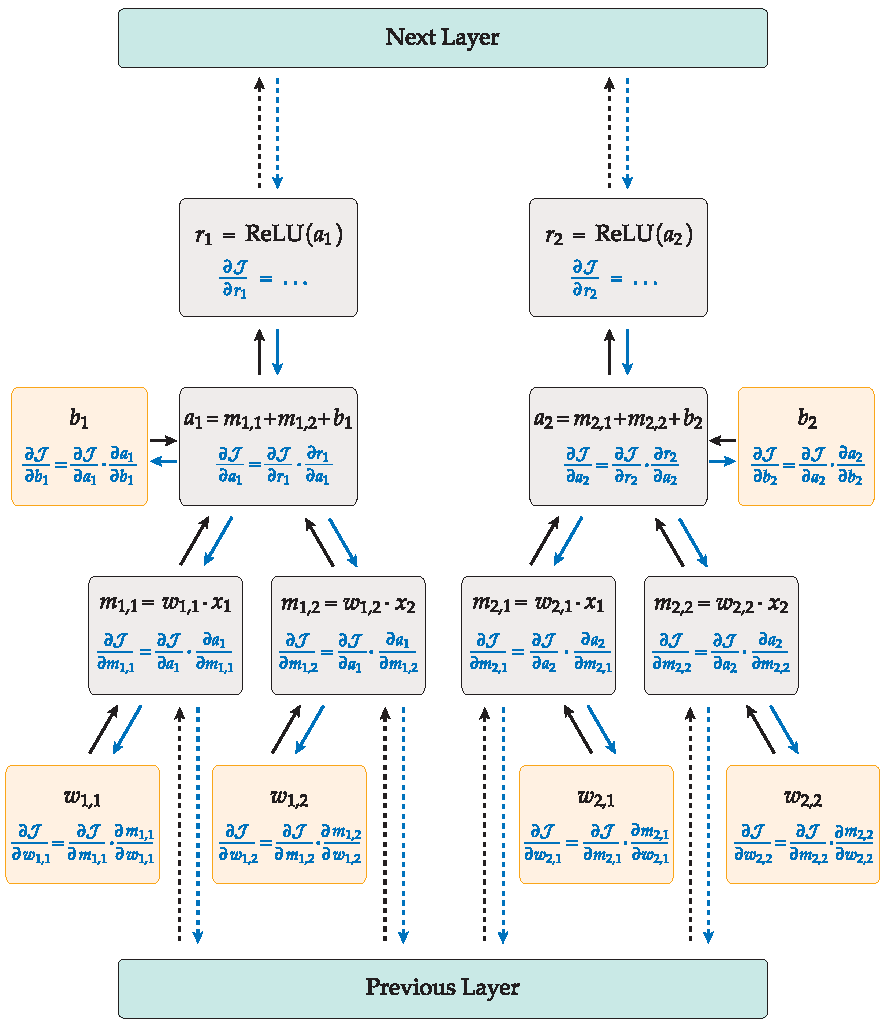
\includegraphics[height=0.85\textheight]{figures/backprop.pdf}
    \caption[Backward Pass on a Computation Graph]
    {Backward Pass on the computation graph of a 
    feed-forward network. The graph
    shows a hidden layer with two neurons. 
    The direction of the backward pass and the partial
    derivatives computed by the backpropagation algorithm
    are shown in blue. Orange nodes are the trainable 
    parameters of the layer. 
    }
    \label{figure:backprop}
\end{figure}

% locally computes the partial derivatives 
% of $\mathcal{J}$ w.r.t each of its parameters according to
% the chain rule using the gradients passed in from the higher 
% layer and finally passes the result to the next lower 
% layer.
% the backpropagation 
% algorithm \parencite{backprop}. 

Since the gradient gives the ascent direction
of the objective function, \ac{SGD} moves
 $\bm{\theta}$ in the 
opposite direction
by a certain step size $\eta$, which
is called the \textit{learning rate}. 
\autoref{equation:sgd} gives the parameter update 
of \ac{SGD}:
\begin{equation} \label{equation:sgd}
    \bm{\theta}_{t+1} = \bm{\theta}_t - \eta \cdot \nabla_{\bm{\theta}} \mathcal{J}(\bm{\theta})
\end{equation} 

The learning rate $\eta$ is a \textit{hyperparameter}
of the algorithm, meaning the choice for its value needs
to be made before applying the algorithm and plays a 
crucial role in its effectiveness: 
If the learning rate is too low, convergence to the minimum
will be too slow, whereas if it is too high, the algorithm 
might oscillate around the minimum and fail to converge. 
It can be beneficial to change the learning rate during
training such that we begin training with a larger 
learning rate to rapidly approach the minimum and 
gradually decrease the learning rate as training goes on 
to get as close to the 
minimum as possible with smaller adjustments. This can be 
achieved by using a learning rate scheduler, a function 
that returns a multiplier for $\eta$ at each step. 
The learning rate $\eta$ in \autoref{equation:sgd} can 
then be replaced by $\eta_t$, the effective learning rate
at step $t$.

\ac{SGD} is an online algorithm, which means it does not
need to process the entire input outright but can go 
through the input example by example 
\parencite[Chapter 5]{jurafsky}. Usually, inputs are
given in small groups called mini-batches:
% where the batch size is also a hyperparameter. 
In each iteration, $b$ randomly-picked samples are given as
input to the model to calculate $b$ outputs, and 
loss is averaged over the $b$ samples:
\begin{equation}
    \nabla_{\bm{\theta}} \mathcal{J}(\bm{\theta}) = 
    \frac{1}{b}\sum_{i=1}^{b}
    \nabla_{\bm{\theta}} \mathcal{J}_i(\bm{\theta})
    \;;\quad
    \mathcal{J}_i(\bm{\theta}) = \mathcal{J}(\bm{\theta}; \mathbf{x}_i, \mathbf{y}_i)
\end{equation} 
The batch size $b$ is also a hyperparameter. Smaller
batch sizes make noisy updates because of a greater 
variance in the gradients
(in the extreme case of $b=1$, parameters are updated to fit a 
single sample in each iteration). 
Larger batch sizes allow the use of larger 
learning rates while achieving the same optimal 
error bounds \parencite{minibatch} and improve
parallelism as the increased amount of computation per 
iteration can be effectively distributed. On the other hand,
they increase the memory requirement of the algorithm and  
when batch size is too high, it can 
impair the model's ability to generalize:
It has been observed that 
when using larger batch sizes, 
algorithms tend to converge 
to \textit{sharp} minimizers where the  
function increases rapidly in a small neighborhood of 
the minimum, which negatively impacts generalization 
\parencite{minibatch2}.  

\subsection{Adaptive Gradient Methods}
For efficient optimization, one needs to overcome 
a central issue of the \ac{SGD} algorithm, which is its 
slow convergence rate. As discussed in \autoref{section:sgd}, 
the convergence rate is directly bound to the learning rate $\eta$, 
but the algorithm fails to converge when $\eta$ is too high.
Thus, $\eta$ needs to be picked conservatively to avoid
divergence, resulting in excessively slow
convergence rates. Adaptive gradient methods try to solve
this issue by taking the parameter updates 
from previous iterations into account
when calculating the update 
for the current iteration. 

\subsubsection{Momentum}

Ideally, we want to take larger steps
in a direction when a sequence of previous 
gradients all pointed in that direction, effectively
accumulating gradients over time. This is the main idea
behind the momentum method \parencite{momentum-polyak}.
The momentum method calculates a velocity vector 
$\mathbf{v}$ that 
accumulates in directions that persistently reduce 
the objective function across iterations:
\begin{equation}
    \mathbf{v}_{t+1} = \beta \cdot \mathbf{v}_t - \eta \cdot \nabla_{\bm{\theta}}\mathcal{J}(\bm{\theta}_t)
\end{equation}
where $\beta \in \mathbb{R}$ is called the momentum coefficient and determines
the rate of velocity accumulation. The parameter update 
is then given using the velocity vector:
\begin{equation}
    \bm{\theta}_{t+1} = \bm{\theta}_t + \mathbf{v}_{t+1}
\end{equation}

\subsubsection{Nesterov Momentum}

Nesterov’s Accelerated Gradient, also called Nesterov 
momentum \parencite{nesterov}, is a simple modification of
the classical momentum method that has been observed to
increase stability and improve performance 
\parencite{momentum-sutskever}. Instead of computing 
the velocity using the gradient from the current
position, it first performs a partial update and uses the
gradient at the position $\bm{\theta}_t + \beta \cdot \mathbf{v}_t$:
\begin{equation}
    \mathbf{v}_{t+1} = \beta \cdot \mathbf{v}_t - \eta \cdot \nabla_{\bm{\theta}}\mathcal{J}(\bm{\theta}_t + \beta \cdot \mathbf{v}_t)
\end{equation}

\subsubsection{Adam}

The last adaptive gradient method we want to share is Adam
\parencite{adam}. Adam computes two moving averages
similar to momentum:  
\begin{equation}
    \mathbf{m}_{t+1} = \beta_1 \cdot \mathbf{m}_t + (1 - \beta_1) \cdot \nabla_{\bm{\theta}} \mathcal{J}(\bm{\theta}_{t})
\end{equation}
\begin{equation}
    \mathbf{v}_{t+1} = \beta_2 \cdot \mathbf{v}_t + (1 - \beta_2) \cdot (\nabla_{\bm{\theta}} \mathcal{J}(\bm{\theta}_{t}))^2
\end{equation}
where $\mathbf{m}$ and $\mathbf{v}$ operate as
estimates of the mean and 
the uncentered variance of the gradient respectively
and $\beta_1, \beta_2 \in [0, 1)$ control their decay rates.
$\mathbf{m}_0$ and $\mathbf{v}_0$ are initialized as 
0's, which cause a bias towards 0, especially in the 
early steps and when $\beta_1$ and $\beta_2$ are close to
1. Thus, a bias correction is applied:
\begin{equation}
    \hat{\mathbf{m}}_{t+1} = \frac{1}{1 - \beta_1^{t+1}}\mathbf{m}_{t+1}
\end{equation}
\begin{equation}
    \hat{\mathbf{v}}_{t+1} = \frac{1}{1 - \beta_2^{t+1}}\mathbf{v}_{t+1}
\end{equation}
Finally, parameters are updated using the bias-corrected 
estimates:
\begin{equation}
    \bm{\theta}_{t+1} = \bm{\theta}_t - \eta \cdot \frac{\hat{\mathbf{m}}_{t+1}}{\sqrt{\hat{\mathbf{v}}_{t+1}} + \epsilon}
\end{equation}
where $\epsilon > 0$ is a very small number. The authors 
give $\beta_1 = 0.9$, $\beta_2 = 0.999$ and 
$\epsilon = 10^{-8}$ as good default settings with
$\eta = 0.001$.

\subsection{Finite Difference Methods}
Finite difference methods are 
zeroth-order methods that solve an optimization problem
using the same recipe as first-order gradient methods, only
without explicit computation of a gradient. Instead, 
gradients are estimated from a sequence of 
function evaluations, effectively requiring only forward
passes to train a neural network.

The Kiefer-Wolfowitz finite-difference algorithm
\parencite{KieferWolfowitz} approximates the derivative 
of a function $f(x)$ as
\begin{equation}\label{equation:finitediff}
    f'(x) \approx \frac{f(x+h)-f(x-h)}{2h}
\end{equation}
The quantity $h$ is 
called the finite difference interval and using the 
Taylor series expansion, the following relation 
can be shown for
sufficiently small intervals
\parencite[Page 54]{optimizationbook2}:
\begin{equation}
    \frac{f(x+h)-f(x-h)}{2h} = f'(x) + O(h^2)
\end{equation}
Using the Kiefer-Wolfowitz finite difference, we can obtain 
a gradient approximation $\hat{\nabla}\mathcal{J}(\bm{\theta})$:
\begin{equation}
    \hat{\nabla}_i \mathcal{J}(\bm{\theta}) = \frac{\mathcal{J}(\bm{\theta} + h \cdot \mathbf{e}_i) - \mathcal{J}(\bm{\theta} - h \cdot \mathbf{e}_i)}{2h}
\end{equation} 
\begin{equation}
    \hat{\nabla} \mathcal{J}(\bm{\theta}) = (\hat{\nabla}_1 \mathcal{J}(\bm{\theta}), \hat{\nabla}_2 \mathcal{J}(\bm{\theta}), \dots, \hat{\nabla}_n \mathcal{J}(\bm{\theta}))^T
\end{equation} 
where $\mathbf{e}_i$ is the $i$-th unit vector. The disadvantage of this method is the 
large number of function evaluations it requires 
($2n$ evaluations for $n$-dimensional $\bm{\theta})$
\parencite{finitediffpaper}. 

\ac{SPSA} \parencite{spsa} reduces the number of function
evaluations to 2 by perturbing all directions at the 
same time: 
\begin{equation} \label{equation:spsa}
    \hat{\nabla} \mathcal{J}(\bm{\theta}) = \frac{\mathcal{J}(\bm{\theta} + h\cdot\mathbf{z}) - \mathcal{J}(\bm{\theta} - h\cdot\mathbf{z})}{2h} \cdot \mathbf{z}
\end{equation}
where $\mathbf{z} \in \mathbb{R}^n$ is a vector of small 
random perturbations and can be sampled, e.g.\ 
from a standard gaussian
distribution with $z_i \sim \mathcal{N}(0, 1)$.
Using the gradient estimate from \autoref{equation:spsa}
as a replacement for the gradient in \autoref{equation:sgd}
(\ac{SGD}),
we obtain the \textbf{ZO-SGD} algorithm \parencite{spsa}.

The \textbf{ZO-signSGD} algorithm \parencite{zosignsgd} 
instead uses the sign
of the estimated gradient as direction for the update.
It has been shown that the first-order signSGD 
algorithm \parencite{signsgd}
yields an empirically faster convergence speed than standard 
\ac{SGD} 
% as taking the sign of the gradient can mitigate 
% the negative effect of gradient noise of large variance. 
ZO-signSGD shows analogous improvements in 
convergence rate over ZO-SGD. However, it has worse 
convergence accuracy than ZO-SGD as it only converges 
to a neighborhood of the minimum \parencite{zoadamm}.

\textbf{MeZO} \parencite{mezo} proposes a memory-efficient 
implementation of ZO-SGD where the algorithm does not store 
the random perturbation vector 
$\mathbf{z}$ of \autoref{equation:spsa}. Instead, 
the random seed is stored and the random number generator
is reset by this seed to resample $\mathbf{z}$ for each 
of its uses, giving a
memory footprint equivalent to the inference memory cost.

The zeroth-order adaptive momentum method (\textbf{ZO-AdaMM})
\parencite{zoadamm} implements an adaptive gradient method
using the zeroth-order gradient estimate. It fuses the 
gradient estimate with AMSGrad 
\parencite{amsgrad}, which is a modified version of Adam. 
Compared to other zeroth-order methods, 
the authors show superior performance and convergence rate 
for the task of designing adversarial examples. 

% Consider the definition of the derivative 
% of a function $f(x)$: 
% \begin{equation}\label{equation:finitediff}
%     f'(x) = \lim_{h \rightarrow 0} \frac{f(x+h)-f(x)}{h}
% \end{equation}
% The difference $f(x+h) - f(x)$ of function evaluations is 
% called a finite difference and can be used to estimate 
% the gradient of $f$ at a point $x$ \parencite{optimizationbook}.
% The quantity $h$ is 
% called the finite difference interval. Instead of 
% calculating the derivative analytically as the limit, one 
% can approximate the derivative by using a 
% small finite
% difference interval. Using the Taylor series expansion, 
% \textcite[Section 2.3.5]{optimizationbook2} show the following 
% relation for sufficiently small $h$: 
% \begin{equation}
%     \frac{f(x+h)-f(x)}{h} = f'(x) + O(h) 
% \end{equation}

\subsection{Direct Search Methods} \label{section:directsearch}
% Under direct search methods we will present zeroth-order 
% methods that do not use an approximation of the gradient.
Unlike the previously discussed finite difference 
methods, direct search methods do not rely on a 
gradient approximation.
Instead, they conduct a search by identifying 
possible candidates $\bm{\hat{\theta}}_1, \dots \bm{\hat{\theta}}_c$, 
for the parameter vector $\bm{\theta}$, 
evaluating the objective function $\mathcal{J}$ 
on those points and updating the parameters 
to the best candidate: 
\begin{equation}
    \bm{\theta}_{t+1} = \arg\min_{\bm{\hat{\theta}}} \{\mathcal{J}(\bm{\hat{\theta}}) | \bm{\hat{\theta}} \in \{\bm{\hat{\theta}}_1, \dots, \bm{\hat{\theta}}_c\}\}
\end{equation}
Typically, a candidate
is determined by adding a random perturbation vector to
the current parameter: 
\begin{equation}
    \bm{\hat{\theta}}_k = \bm{\theta}_t + \mathbf{z}_k \;;\quad \mathbf{z}_k \sim \mathcal{D}_k 
\end{equation}
where $\mathcal{D}_k$ is some sampling distribution.

% We refer to \textcite{directsearch} for some 
% important properties of direct search methods: 
% We refer to \textcite{directsearch} to present the 
% strengths and weaknesses of direct search methods:
\textcite{directsearch} give a detailed review of 
the strengths and weaknesses of direct search methods:
Direct search algorithms are usually straightforward to 
implement but have slower convergence rates. Since they 
only need to identify optimal parameters in a small 
search space, 
direct search algorithms can be used to optimize noisy 
or non-smooth functions
where a finite difference approximation of the gradient 
cannot be found reliably, as well as nonnumerical functions
where gradient calculation or estimation is impossible.
Even though asymptotic convergence rates are slow, 
direct search methods can still be applied in practice 
when reaching a sufficiently good solution is more 
important than convergence, particularly when the function 
to optimize is inaccurate. A major limitation of direct 
search methods is that their performance deteriorates 
significantly as the number of variables increases. 
Seeking for ways to overcome this limitation is 
a key part of our work.

\aclu{STP} (\textbf{\acs{STP}}) \parencite{stp}
% considers three candidates per iteration: 
% $\bm{\theta}_t$, $\bm{\theta}_t + \mathbf{z}_k$ 
% and $\bm{\theta}_t + \mathbf{z}_k$ with 
% $\mathbf{z}_k \sim r_k \mathcal{D}$ for a fixed 
% distribution $\mathcal{D}$ and step size $r_k$.
samples a single perturbation vector at each iteration
with $\mathbf{z}_t \sim r_t\mathcal{D}$ where $r_t$ is the step size
at iteration $t$. Then, it considers three points 
for the parameter update: 
\begin{equation}
    \bm{\theta}_{t+1} = \arg\min \{\mathcal{J}(\bm{\theta}_t), \mathcal{J}(\bm{\theta}_t + \mathbf{z}_t), \mathcal{J}(\bm{\theta}_t - \mathbf{z}_t) \}
    % \bm{\theta}_{t+1} = \arg\min \{\mathcal{J}(\bm{\theta}) | \bm{\theta} = \bm{\theta}_t, \bm{\theta} = \bm{\theta}_t + \mathbf{z}, \bm{\theta} = \bm{\theta}_t - \mathbf{z}\}
\end{equation}
% Unlike \ac{GLD}, where the number of additional 
% function evaluations 
% $K$ depends on the size of the search interval with
% $K=\log_2(R/r)$, \ac{STP} only requires 
% On top of the current iterate, \ac{STP} only requires 
% $K=2$ additional function evaluations per iteration, 
% unlike \ac{GLD}, where this number depends 
% on the size of the binary search interval with
% $K=\log_2(R/r)$.
Thus, \ac{STP} only requires 
two additional function evaluations per iteration.

Stochastic Momentum Three Points (\textbf{SMTP}) \parencite{smtp}
is a modification of the \ac{STP} algorithm.
Motivated by the
efficiency of momentum methods in first-order optimization, 
the authors introduce momentum to \ac{STP} and 
demonstrate that momentum could be beneficial
for stochastic zeroth-order methods as well. 

\aclu{GLD} (\textbf{\acs{GLD}}) \parencite{gld} is a simple direct 
search algorithm that
samples random perturbation vectors from a fixed
distribution $\mathcal{D}$ but with different choices of 
radius $r_k$. Given a maximal radius $R$ and a 
minimal radius $r$, the algorithm performs a binary 
search in the interval $[r, R]$ where $r_0 = R$ and 
each consecutive candidate halves the search radius 
until the minimal radius is reached: 
\begin{equation}
    \mathbf{z}_k \sim r_k \mathcal{D} \;;\quad r_k = 2^{-k} R
\end{equation}
The parameter is updated to the best candidate if at least
one of them improves the objective:
\begin{equation}
    % \bm{\theta}_{t+1} = \arg\min_{\bm{\theta}} \{\mathcal{J}(\bm{\theta}) | \bm{\theta} = \bm{\theta}_t, \bm{\theta} = \bm{\theta}_t + \mathbf{z}_k\}
    \bm{\theta}_{t+1} = \arg\min_{\bm{\theta}} \{\mathcal{J}(\bm{\theta} + \mathbf{c}) \mid \mathbf{c} = \mathbf{0}, \mathbf{z}_0, \dots \mathbf{z}_n\}
\end{equation}
This binary search arrangement
allows the authors to give convergence guarantees
depending on the search interval $[r, R]$
when minimizing arbitrary functions.

Although the update rule is similar to \ac{STP}, 
for \ac{GLD}, 
the number of function evaluations per step 
depends on the size of the search interval 
with $K=\log_2(R/r)$, i.e.\ it can be adjusted 
by changing the search interval where larger intervals
perform more function evaluations per iteration but 
give better convergence guarantees. Particularly, a 
smaller minimal radius guarantees convergence to a 
closer neighborhood of the minimum \parencite{gld}. 

\ac{GLD} provides the base algorithm of our work. 
We add our own modifications on top of the 
base \ac{GLD} algorithm for the purpose of using it as 
an optimizer for a neural network model. Above all, this involves an 
effort to overcome the limitations 
on the number of parameters. 
Our methods will be detailed in \autoref{chapter:methods}.

% \begin{equation}
%     \mathbf{v}_{t+1, +} = \beta \mathbf{v}_t + \mathbf{z}_t; \mathbf{v}_{t+1, -} = \beta \mathbf{v}_t - \mathbf{z}_t 
% \end{equation}
% \begin{equation}
%     \bm{\theta}_{t+1, +} = \bm{\theta}_t - r_t \mathbf{v}_{t+1, +}; \bm{\theta}_{t+1, -} = \bm{\theta}_t - r_t \mathbf{v}_{t+1, -}
% \end{equation}
% \begin{equation}
    
% \end{equation}

\section{Importance of Network Parameters} \label{section:fisher}
Neural Networks can fit a wide variety of functions 
thanks to their strong parameterization. However, 
not all parameters are equally important for 
the performance of a network. Having information
about the importance of parameters can be useful as
unimportant parameters can be removed to prune
the network, reducing its size. 

The magnitude of a
parameter is a good indicator of its importance since
parameters with low absolute values will have little 
effect on the output of their respective layers. 
This importance measure allows
connections with weights below a certain threshold 
to be removed from the network without losing 
performance \parencite{weight-pruning}.

The \ac{FIM} is a useful quantity in statistics that 
provides an estimate of the amount of information a random
variable carries about a parameter of its distribution.
For a neural network with parameters $\bm{\theta}$,
the \ac{FIM} is given as
\begin{equation}\label{equation:fisher}
    F_{i,j}(\bm{\theta}) = E\left[\pdv{\log p(\mathbf{x}; \bm{\theta})}{\theta_i} \pdv{\log p(\mathbf{x}; \bm{\theta})}{\theta_j}\right]
\end{equation}
where $p$ is a probability distribution of model
outputs with the given parameters. The \ac{FIM} 
can be used as an importance measure for model parameters.
\textcite{fisher-reduction} show 
that network complexity can be reduced
without a noticeable effect on performance by removing 
parameters with low entries on the diagonal of
the \ac{FIM}.

Computing the \ac{FIM} as given in \autoref{equation:fisher}
requires estimating the probability distribution function
$p$, which is mostly unknown. 
% Therefore, the authors use 
% the method proposed by \tetcite{fisher}, which gives
% an estimate directly from sampled data. 
Therefore, the authors define a method to estimate 
only the diagonal entries of the \ac{FIM}: 
The algorithm iterates over each parameter in $\bm{\theta}$.
Each iteration calculates a perturbation 
$\tilde{\bm{\theta}}$ of the parameter vector where a small 
random perturbation $z$ is added to only the current iterate:
\begin{equation*}
    \tilde{\bm{\theta}} = \bm{\theta} 
\end{equation*}
\begin{equation}
    \tilde{\bm{\theta}}(i) = \tilde{\bm{\theta}}(i) + z
\end{equation}
The algorithm then computes the $D_\alpha$-divergence of 
2 different model outputs: One with the original parameters 
$\bm{\theta}$, the other with the 
perturbed parameters $\tilde{\bm{\theta}}$. 
The divergence is a measure of distance between the 2
distributions described by the 2 model outputs and is 
therefore used as an estimation for the importance of
the iterate. 

The $D_\alpha$-divergence is given by 
\begin{equation}
    D_\alpha(p, q) = \frac{1}{4\alpha(1-\alpha)} \times \left[\int \frac{(\alpha p(\mathbf{x}) - (1-\alpha)q(\mathbf{x}))^2}{\alpha p(\mathbf{x}) + (1-\alpha)q(\mathbf{x})}d\mathbf{x} - (2\alpha-1)^2 \right]
\end{equation}
\textcite{fisher} provide a method to estimate the 
$D_\alpha$-divergence, which is crucial for the importance
estimation algorithm. The method involves constructing
an Euclidean minimal spanning tree of from all points 
$\mathbf{X}_p, \mathbf{X}_q$ sampled from the 
2 distributions $p$ and $q$. The number of edges 
connecting a point from $p$ to a point from $q$ gives
the Friedman-Rafsky multi-variate two sample test statistic
$\mathcal{C}(\mathbf{X}_p, \mathbf{X}_q)$
\parencite{fm}. An estimation for the $D_\alpha$-divergence
can then be computed as
\begin{equation}
    D_\alpha(p, q) \approx 1 - \mathcal{C}(\mathbf{X}_p, \mathbf{X}_q) \frac{N_p + N_q}{2N_pN_q}
\end{equation}
where $N_p$ and $N_q$ are the number of samples from $p$ 
and $q$. Finally, taking $p$ and $q$ as distributions modeled by 2 
neural networks with parameters $\bm{\theta}$ and
$\tilde{\bm{\theta}}$ with 
$\mathbf{X}_p$ and $\mathbf{X}_q$ being the sampled model 
outputs, one can estimate the $D_\alpha$-divergence,
which gives an estimation for 
the importance of the perturbed parameter.
% The importance estimation algorithm has to estimate the 
% $D_\alpha$-divergence of the 2 outputs. 

% The algorithm adds a small 
% random perturbation to each parameter in $\bm{\theta}$
% and calculates the model output with the perturbed 
% parameters. Then, it calculates the $D_\alpha$-divergence
% of this output with the output original 
